
\let\negmedspace\undefined
\let\negthickspace\undefined
\documentclass[journal,12pt,twocolumn]{IEEEtran}
%\documentclass[conference]{IEEEtran}
%\IEEEoverridecommandlockouts
% The preceding line is only needed to identify funding in the first footnote. If that is unneeded, please comment it out.
\usepackage{cite}
\usepackage{amsmath,amssymb,amsfonts,amsthm}
\usepackage{algorithmic}
\usepackage{graphicx}
\usepackage{textcomp}
\usepackage{xcolor}
\usepackage{txfonts}
\usepackage{listings}
\usepackage{enumitem}
\usepackage{mathtools}
\usepackage{gensymb}
\usepackage[breaklinks=true]{hyperref}
\usepackage{tkz-euclide} % loads  TikZ and tkz-base
\usepackage{listings}
\usepackage{placeins}
%
%\usepackage{setspace}
%\usepackage{gensymb}
%\doublespacing
%\singlespacing

%\usepackage{graphicx}
%\usepackage{amssymb}
%\usepackage{relsize}
%\usepackage[cmex10]{amsmath}
%\usepackage{amsthm}
%\interdisplaylinepenalty=2500
%\savesymbol{iint}
%\usepackage{txfonts}
%\restoresymbol{TXF}{iint}
%\usepackage{wasysym}
%\usepackage{amsthm}
%\usepackage{iithtlc}
%\usepackage{mathrsfs}
%\usepackage{txfonts}
%\usepackage{stfloats}
%\usepackage{bm}
%\usepackage{cite}
%\usepackage{cases}
%\usepackage{subfig}
%\usepackage{xtab}
%\usepackage{longtable}
%\usepackage{multirow}
%\usepackage{algorithm}
%\usepackage{algpseudocode}
%\usepackage{enumitem}
%\usepackage{mathtools}
%\usepackage{tikz}
%\usepackage{circuitikz}
%\usepackage{verbatim}
%\usepackage{tfrupee}
%\usepackage{stmaryrd}
%\usetkzobj{all}
%    \usepackage{color}                                            %%
%    \usepackage{array}                                            %%
%    \usepackage{longtable}                                        %%
%    \usepackage{calc}                                             %%
%    \usepackage{multirow}                                         %%
%    \usepackage{hhline}                                           %%
%    \usepackage{ifthen}                                           %%
  %optionally (for landscape tables embedded in another document): %%
%    \usepackage{lscape}     
%\usepackage{multicol}
%\usepackage{chngcntr}
%\usepackage{enumerate}

%\usepackage{wasysym}
%\newcounter{MYtempeqncnt}
\DeclareMathOperator*{\Res}{Res}
%\renewcommand{\baselinestretch}{2}
\renewcommand\thesection{\arabic{section}}
\renewcommand\thesubsection{\thesection.\arabic{subsection}}
\renewcommand\thesubsubsection{\thesubsection.\arabic{subsubsection}}

\renewcommand\thesectiondis{\arabic{section}}
\renewcommand\thesubsectiondis{\thesectiondis.\arabic{subsection}}
\renewcommand\thesubsubsectiondis{\thesubsectiondis.\arabic{subsubsection}}

% correct bad hyphenation here
\hyphenation{op-tical net-works semi-conduc-tor}
\def\inputGnumericTable{}                                 %%

\lstset{
%language=C,
frame=single, 
breaklines=true,
columns=fullflexible
}
%\lstset{
%language=tex,
%frame=single, 
%breaklines=true
%}

\begin{document}
%


\newtheorem{theorem}{Theorem}[section]
\newtheorem{problem}{Problem}
\newtheorem{proposition}{Proposition}[section]
\newtheorem{lemma}{Lemma}[section]
\newtheorem{corollary}[theorem]{Corollary}
\newtheorem{example}{Example}[section]
\newtheorem{definition}[problem]{Definition}
%\newtheorem{thm}{Theorem}[section] 
%\newtheorem{defn}[thm]{Definition}
%\newtheorem{algorithm}{Algorithm}[section]
%\newtheorem{cor}{Corollary}
\newcommand{\BEQA}{\begin{eqnarray}}
\newcommand{\EEQA}{\end{eqnarray}}
\newcommand{\define}{\stackrel{\triangle}{=}}

\bibliographystyle{IEEEtran}
%\bibliographystyle{ieeetr}


\providecommand{\mbf}{\mathbf}
\providecommand{\pr}[1]{\ensuremath{\Pr\left(#1\right)}}
\providecommand{\qfunc}[1]{\ensuremath{Q\left(#1\right)}}
\providecommand{\sbrak}[1]{\ensuremath{{}\left[#1\right]}}
\providecommand{\lsbrak}[1]{\ensuremath{{}\left[#1\right.}}
\providecommand{\rsbrak}[1]{\ensuremath{{}\left.#1\right]}}
\providecommand{\brak}[1]{\ensuremath{\left(#1\right)}}
\providecommand{\lbrak}[1]{\ensuremath{\left(#1\right.}}
\providecommand{\rbrak}[1]{\ensuremath{\left.#1\right)}}
\providecommand{\cbrak}[1]{\ensuremath{\left\{#1\right\}}}
\providecommand{\lcbrak}[1]{\ensuremath{\left\{#1\right.}}
\providecommand{\rcbrak}[1]{\ensuremath{\left.#1\right\}}}
\theoremstyle{remark}
\newtheorem{rem}{Remark}
\newcommand{\sgn}{\mathop{\mathrm{sgn}}}
\providecommand{\abs}[1]{\left\vert#1\right\vert}
\providecommand{\res}[1]{\Res\displaylimits_{#1}} 
\providecommand{\norm}[1]{\left\lVert#1\right\rVert}
%\providecommand{\norm}[1]{\lVert#1\rVert}
\providecommand{\mtx}[1]{\mathbf{#1}}
\providecommand{\mean}[1]{E\left[ #1 \right]}
\providecommand{\fourier}{\overset{\mathcal{F}}{ \rightleftharpoons}}
%\providecommand{\hilbert}{\overset{\mathcal{H}}{ \rightleftharpoons}}
\providecommand{\system}{\overset{\mathcal{H}}{ \longleftrightarrow}}
	%\newcommand{\solution}[2]{\textbf{Solution:}{#1}}
\newcommand{\solution}{\noindent \textbf{Solution: }}
\newcommand{\cosec}{\,\text{cosec}\,}
\providecommand{\dec}[2]{\ensuremath{\overset{#1}{\underset{#2}{\gtrless}}}}
\newcommand{\myvec}[1]{\ensuremath{\begin{pmatrix}#1\end{pmatrix}}}
\newcommand{\mydet}[1]{\ensuremath{\begin{vmatrix}#1\end{vmatrix}}}
%\numberwithin{equation}{section}
%\numberwithin{equation}{subsection}
%\numberwithin{problem}{section}
%\numberwithin{definition}{section}
%\makeatletter
%\@addtoreset{figure}{problem}
%\makeatother

%\let\StandardTheFigure\thefigure
\let\vec\mathbf
%\renewcommand{\thefigure}{\theproblem.\arabic{figure}}
%\renewcommand{\thefigure}{\theproblem}
%\setlist[enumerate,1]{before=\renewcommand\theequation{\theenumi.\arabic{equation}}
%\counterwithin{equation}{enumi}


%\renewcommand{\theequation}{\arabic{subsection}.\arabic{equation}}

%\def\putbox#1#2#3{\makebox[0in][l]{\makebox[#1][l]{}\raisebox{\baselineskip}[0in][0in]{\raisebox{#2}[0in][0in]{#3}}}}
%     \def\rightbox#1{\makebox[0in][r]{#1}}
%     \def\centbox#1{\makebox[0in]{#1}}
%     \def\topbox#1{\raisebox{-\baselineskip}[0in][0in]{#1}}
%     \def\midbox#1{\raisebox{-0.5\baselineskip}[0in][0in]{#1}}

\vspace{3cm}

\title{
\textbf{Report of Hardware Assignment}\\\large \textbf{Random Number Generation using Shift Registers} \\ \large \textbf{AI1110}: Probability and Random Variables 


}
\author{ Rishitha Surineni\\ cs22btech11050} 


% make the title area
\maketitle

\newpage

%\tableofcontents

\bigskip

\renewcommand{\thefigure}{\theenumi}
\renewcommand{\thetable}{\theenumi}


\section{\textbf{Components}}
\begin{table}[htbp]
\centering
\caption{Components List}

\begin{tabular}{|c|c|c|}
\hline
COMPONENT	&VALUE	&QUANTITY	\\ \hline
Breadboard	&	&1	\\ \hline
Seven Segment Display	&Common Anode	&1	\\ \hline
Decoder	&7447	&1	\\ \hline
Flip Flop	&7474	&2	\\ \hline
X-OR GATE	&7486	&1	\\ \hline
555 IC	&	&1	\\ \hline
Resistor	&1Kilo Ohm	&1	\\ \hline
Resistor	&1Mega Ohm	&1	\\ \hline
Capacitor	&100nF	&1	\\ \hline
Capacitor	&10nF	&1	\\ \hline
Wires	&	&6	\\ \hline
Micro USB	&	&1	\\ \hline
\end{tabular}
\label{Components List}
\end{table}

\section{\textbf{Description}}
The Aim of this experiment is to generate Random Numbers using Shift Registers.
\\\textbf{Shift Register}: A Shift Register is a designed by connecting a set of Flip Flops where each flip flop stores a single bit of data. It is used to store and transfer data.
\\We are using the above mentioned components in the experiment.

\subsection{\textbf{Use of the Components}}
\begin{enumerate}
	\item \textbf{Breadboard}
	\\It is used to build the circuit for the experiment.
	\item \textbf{Seven Segment Display}
	\\It is used to display the generated random Number.
	\item \textbf{Decoder}
	\\It is a 7447 IC which coverts a Binary Coded Decimal inputs into output suitable for 7-Segment Display.
	\item \textbf{Flip Flop}
	\\Each 7474 IC has two flip flops which can store a single bit of data each.
	\item \textbf{X-OR Gate}
	\\It is a 7486 IC.This logic gate is used to generate the random sequence.
	\item \textbf{555 IC}
	\\This IC generates the clock pulses for the shift registers
	\item \textbf{Resistors, Capacitors}
	\\These are used to construct the clock circuit. Changing them changes the frequency of clock circuit and intern changes the speed in which the numbers are displayed.
	\item \textbf{Wires}
	\\To make the connections betwwen the components
	\item \textbf{MicroUSB}
	\\To provide the power supply for the circuit
\end{enumerate}
\subsection{\textbf{Construction of Circuit}}
Firstly, place a Micro USB to get power supply.And give connections for VCC and ground.Then create a clock circuit by using a 555 IC,two capacitors and a resistor.This clock circuit converts the power supply into a square pulse.The frequency of this can be adjusted. Then place the other ICs in the order(7486,7474,7474).Give connections in between these components such that output of clock is given to the two 7474 ICs.These two ICs along with the X-OR gate(7486 IC)
produce the Binary Coded Decimal(with one bit from each flip flop) as output. This output is given to the Decoder(7447 IC). The output of this Decoder is given to the 7 Segment Display.The sequence of Random Numbers is displayed on the 7 Segment Display.

\section{\textbf{CIRCUIT DIAGRAM}}
The below is the image of output from the circuit.
\begin{figure}[htbp]
	\centering
	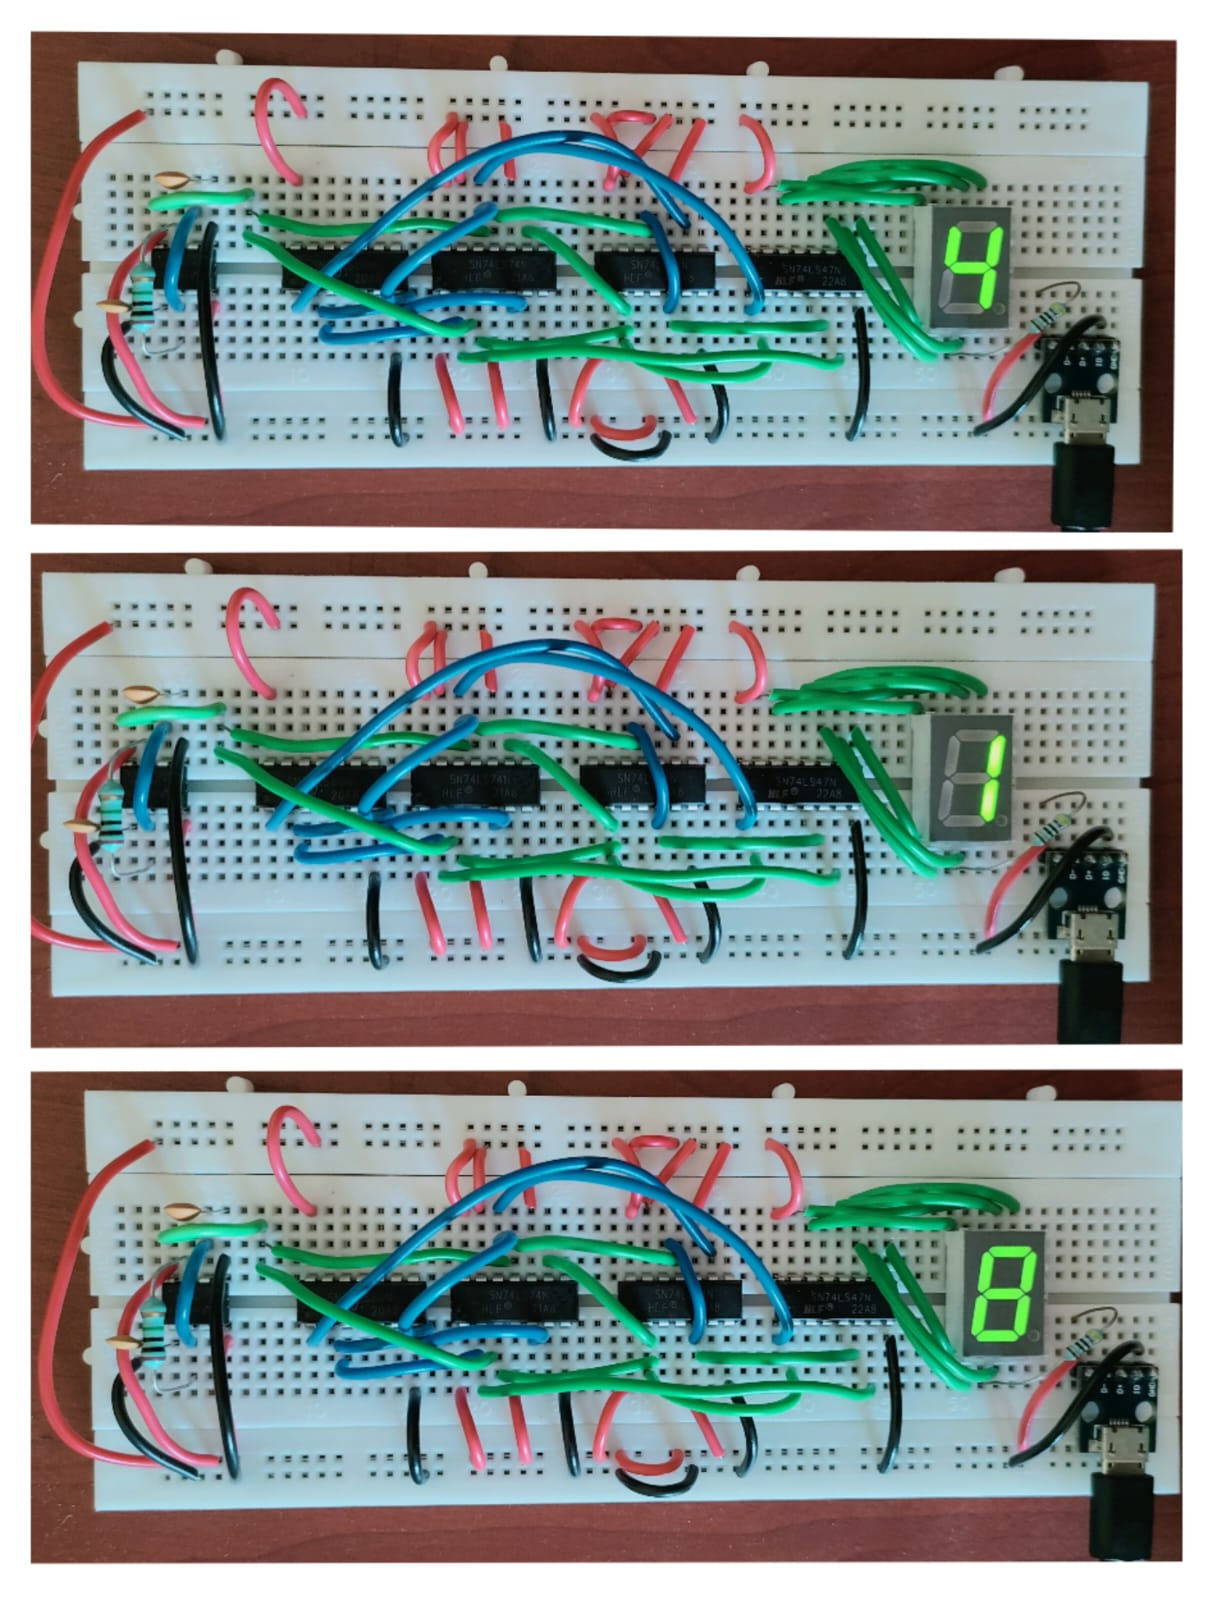
\includegraphics[width=1.5\columnwidth]{Figures/Circuit_Image.jpeg}
	Circuit Diagram
\end{figure}
\clearpage
\begin{figure}[t]
	\centering
	\section{\textbf{BLOCK DIAGRAM}}
	The below is the block diagram for the circuit.
	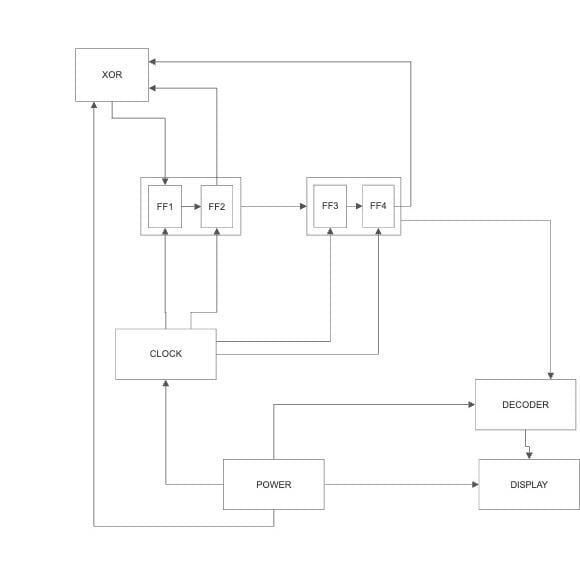
\includegraphics[width=1.5\columnwidth]{Figures/Block_Diagram.jpg}
	Block Diagram
\end{figure}
\end{document}



